% Input immediately after the chapter title/label in chapters/03-design.tex.
% First of the ordered design fragments; architecture starts on body page 1.
% Shared commands and diagram styles are provided by reportstyle.sty.

% Page 1: project overview and overall architecture.
\section{项目概述与总体架构}
“谁能打开你的窗”是一款面向低压力社交场景的交流应用。用户填写个人介绍和相遇偏好后，可以通过相遇卡片浏览候选对象。发现感兴趣的对象时，用户可以先收藏，随后再通过纸条发起联系。

项目采用 B/S 架构，图\ref{fig:design-architecture}给出了各部分的分工。用户在浏览器里操作，Node.js 服务端处理请求，SQLite 保存业务数据。表达建议、虚拟人物回复和立绘生成需要调用外部 AI 服务。

\begin{figure}[H]
\centering
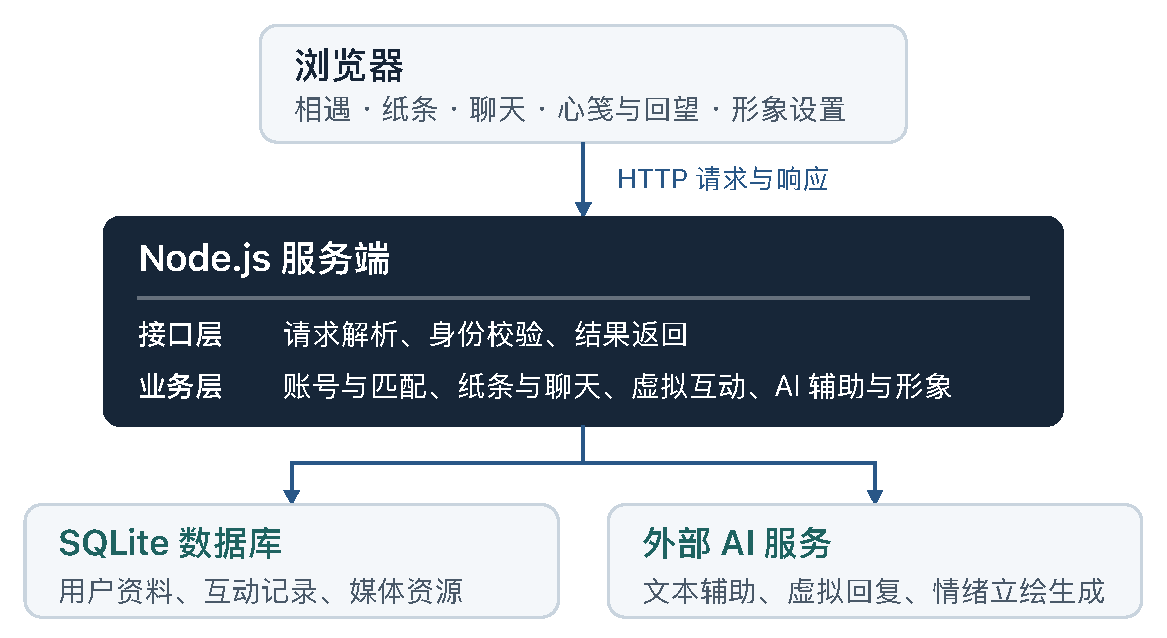
\includegraphics[width=\linewidth]{assets/design/architecture.pdf}
\caption{项目总体架构}\label{fig:design-architecture}
\end{figure}

真人交流分为发现对象、发起联系和建立会话三个阶段。收藏用于保留感兴趣的对象，发纸条则需要用户主动发起。收件人可以根据纸条内容决定是否接受，只有接受并回信后才建立会话。若邀请未获接受，发信人仍可继续浏览其他候选对象。

系统还提供内置人物、心笺和回望。AI 给出的表达建议由用户决定是否采用和发送。生成之类需要等待的操作会显示进度，失败时提示重试。

\clearpage
